\documentclass[]{article}
\usepackage{graphicx}
\usepackage{amsmath}
\usepackage[sort, numbers]{natbib}


%opening
\title{Supplementary Materials for Crystal Hypergraph Convolutional Neural Networks}
\author{Alexander J. Heilman, Weiyi Gong, Qimin Yan}

\begin{document}

\maketitle

\section{Motif Features: Structure Order Parameters \& Continuous Symmetry Measures}
The geometry of the motifs were incorporated as features composed of a concatenated list of structure order parameters and continuous symmetry measures (CSMs) for a set of common local environments. 

Structure order parameters are coordinate system invariant measures of 3 dimensional structure that are designed to be close to one when a given structure is similar to some prototypical arrangement. Note that this isn't in general a true 'distance'-like measure to some shape as a CSM is, however. The list of order parameters included those implemented in pymatgen code and described in \cite{orderparam1, orderparam2}.

A CSM is defined precisely so that it may act as a 'distance' from some prototypical shape to some given structure.

\section{CHGConv}\label{chgconv}
A specific implementation of a hypergraph convolutional operator in the hypergraph message passing framework is a generalization of CGConv implemented in pytorch geometric and based on CGCNN's convolutional operator defined in eq (5) of the original paper.

\begin{align*}
	x_i^{t+1} &= \sum_{b_j} f(x_i^t, b_j,\text{AGG}(\lbrace x_j^t\in b_j \rbrace )) \\ 
	& = \text{BN}\bigg[\sum_{b_j}\sigma \big(W_c\cdot [x_j\oplus b_j\oplus \text{AGG}(\lbrace x_j^t\in b_j \rbrace ] )\big)\\
	&\quad\quad\cdot S^+ (W_f\cdot (x_j\oplus b_j\oplus \text{AGG}(\lbrace x_j^t\in b_j \rbrace ) )  ) \bigg]
\end{align*}
In the model utilized in this work, we generally employed use of a learnable set of common aggregation functions for the neighborhood feature aggregation ($\text{AGG}$ above), inspired by \textit{ChemGNN} \cite{chemgnn}.

\section{Hyperparameters for Testing}\label{app:hyperparam}
For each convolutional structure, testing was done for a model with 3 convolutional layers. Each convolutional layer consists of back-to-back convolution from the smallest to the largest hyperedge type (for example two bond \& motif layers consist of a total sequence of bond, motif bond, motif). 

Stochastic gradient descent (SGD) was used as an optimizer through training with an initial learning rate of 0.01. A multi-step learning rate scheduler divided this learning rate by a factor of 10 at epoch 150, with training running for a total of 300 epochs.  

Hidden node features were of dimension 64 through all convolutional layers, and a hidden output layer of dimension 128 was used (similar to CGCNN's architecture). The loss functions utilized were MSE (for regression tasks) and cross entropy (for classification tasks). Accuracy is then reported in MAE for regression tasks and area under curve (AUC) for classification tasks. 

Results reported were averaged over 5 folds of nested cross-validation. The datasets were divided into 80\% for training and 20\% for test for each fold, with a further 20\% of the training subset being used as an indicative validation set, where the best performance on this dataset was used to select the model applied to the test set. 


\section{Comparison to Line Graph}
A more usual approach for the incorporation of bond angle information is via the construction of a line graph, as in \cite{alignn, m3gnet}. 
\begin{center}
	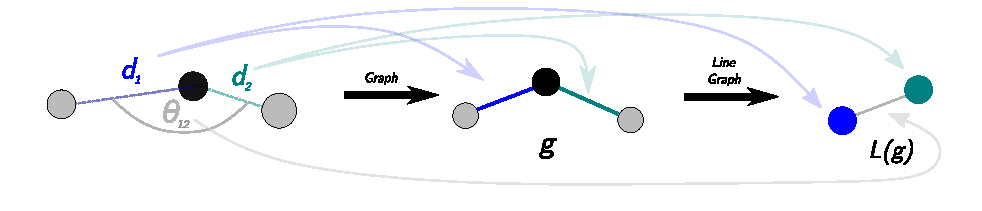
\includegraphics[scale=0.72]{line_graph_ex.pdf}
\end{center}
These models generally first update the edge features of the crystal graph $\mathcal{G}$ by first applying some graph convolutional operator to the line graph $L(\mathcal{G})$ with angles encoded in  $L(\mathcal{G})$'s initial edge features.

Our argument against such representation schemes here is that the order of messages grows combinatorically for derived line graphs as $\mathcal{O}(nm^2)$, where $n$ is the number of nodes and $m$ is the average number of edges per node in $\mathcal{G}$.

Here, we incorporate a similar level of higher-order geometrical structure instead in a local environment, or 'motif', hyperedge (defined below). Note that these include only an extra number of messages on the order $\mathcal{O}(mn)$ if each node in a motif gets a message, or on the order $\mathcal{O}(n)$ if only center nodes are updated by their own motif hyperedges.


\section{Hyperedge Index}
Hypergraphs are treated as a set of node feactures $x$, hyperedge features $h$, and hyperedge indices $I$. 

The hyperedge index is, computationally, treated as a $[2,nm]$ dimensional vector (where $m$ is the number of hyperedges and $n$ is the avereage number of nodes contained in any hyperedge). 
The first index is the node contained and the second index is the containing hyperedge (as in \cite{hypergraphconv}).
\begin{center}
	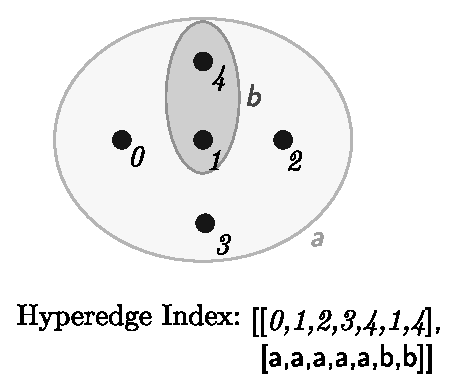
\includegraphics[scale = 1]{hyperedge_index.pdf}
\end{center}

\bibliography{chgcnn} %You need to replace "rsc" on this line with the name of your .bib file
\bibliographystyle{rsc} %the RSC's .bst file

\end{document}
